\chapter {Thực nghiệm và đánh giá mô hình}

\section{Chuẩn bị dữ liệu, nghiên cứu, phân tích đề tài }
\subsection{Chuẩn bị kiến thức nền tảng}
\begin{itemize}
\item Nghiên cứu các công trình liên quan tới đề tài mà mình đang thực hiện.
\item Lựa chọn hướng tiếp cận.
\item Hiểu được căn bản và cách hoạt động của mạng CNN.
\item Hiểu được kiến trúc nâng cao của mạng CNN cũng như các vấn đề và cách giải quyết của nó.
\item Tìm hiểu công cụ sử dụng TensorFlow
\end{itemize}

\subsection{Nghiên cứu kỹ thuật dõi chuyển động mắt hiện nay}
Có hai phương pháp để theo dõi chuyển động mắt hiện nay: Camera Video thông thường và Camera hồng ngoại có đèn LED hồng ngoại. 
Camera hồng ngoại được phát triển vì phản chiếu để định vị mắt  chính xác. Nhưng với sự phát triển của các công nghệ mới, điều này có thể được thay thế bằng một số cách như nhận dạng tính năng bằng cách sử dụng mạng nơ ron thần kinh tích chập (CNNs).

\begin{center}
    \begin{figure}[h!]
    \begin{center}
     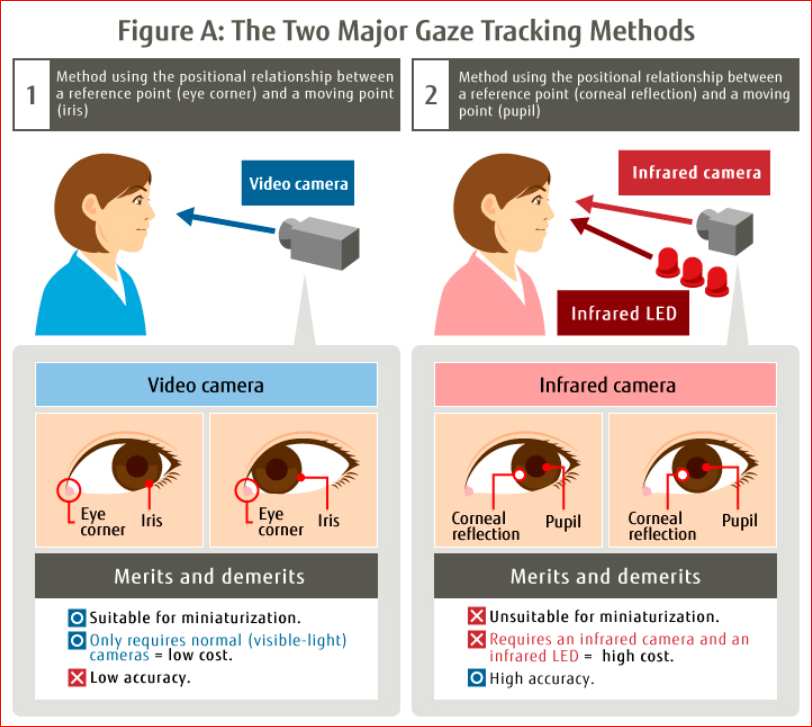
\includegraphics[scale=0.4]{img/Camera.png}
    \end{center}
    \caption{Camera Video thông thường và Camera hồng ngoại có đèn LED hồng ngoại. \cite{eyetrackingapplication}}
    \label{refhinh20}
    \end{figure}
\end{center}

Camera hồng ngoại- có đèn hồng ngoại:  (infrared LED) là camera thông thường được trang bị thêm  các đèn hồng ngoại  có cảm biến ánh sáng tên tiếng anh là (light sensor). Cảm biến này sẽ tự nhảy nếu điều kiện môi trường thiếu sáng, khi bật cảm biến hồng ngoại sẽ bật lên giúp camera quay được những cảnh trong bóng tối giúp hình ảnh chính xác và ổn định nhưng tốn nhiều chi phí hơn camera thông thường.


\begin{center}
    \begin{figure}[h!]
    \begin{center}
     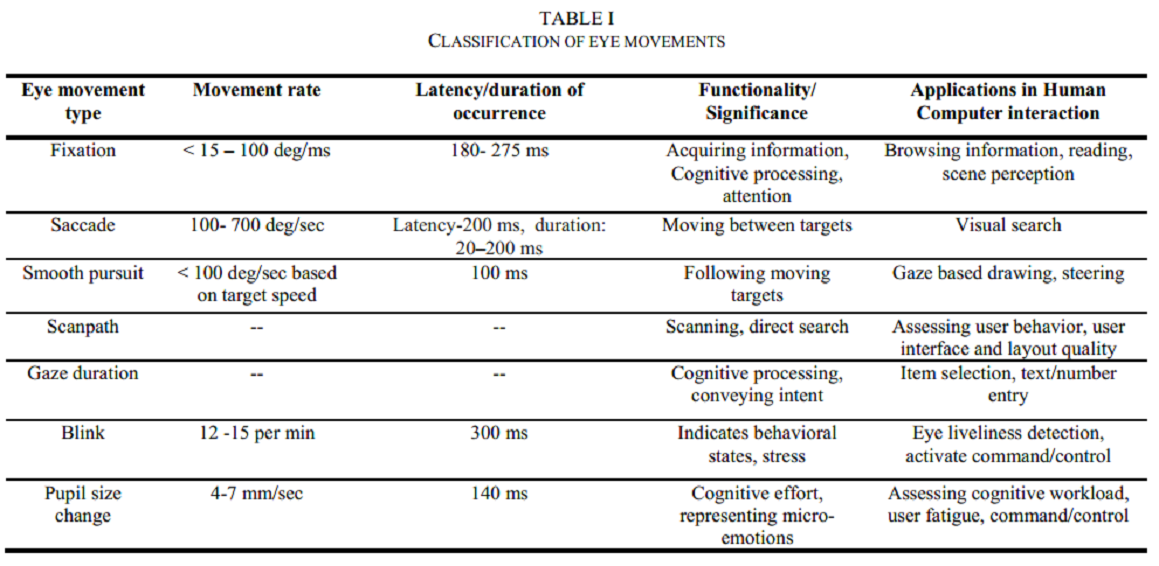
\includegraphics[scale=0.5]{img/Classification_of_eye_movements.png}
    \end{center}
    \caption{Phân loại sự vận động của mắt \cite{AReviewandAnalysisofEyeGazeEstimation}}
    \label{refhinh15}
    \end{figure}
\end{center}

\clearpage 

\begin{center}
    \begin{figure}[h!]
    \begin{center}
     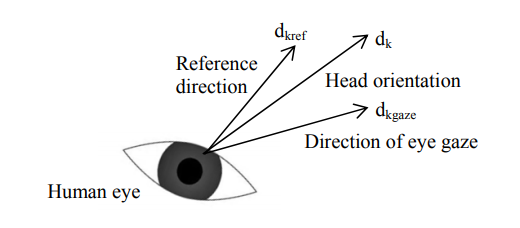
\includegraphics[scale=0.5]{img/Relation_between_gaze_direction_head_pose.png}
    \end{center}
    \caption{Mối quan hệ giữa hướng nhìn và tư thế đầu \cite{AReviewandAnalysisofEyeGazeEstimation}}
    \label{refhinh15}
    \end{figure}
\end{center}

\begin{center}
    \begin{figure}[h!]
    \begin{center}
     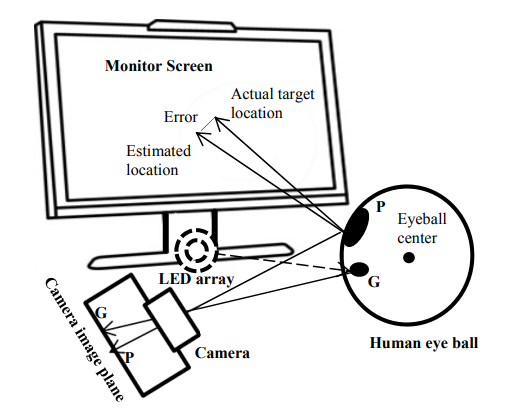
\includegraphics[scale=0.5]{img/Schematic_diagram_of_a_typical_gaze_tracking_system.png}
    \end{center}
    \caption{Sơ đồ của một hệ thống theo dõi hướng nhìn. P là đồng tử của bóng mắt người và G là vị trí phản chiếu được hình thành trên giác mạc, được chụp trên mặt phẳng camera Hình ảnh này cho thấy lỗi trong ước tính ánh nhìn cũng như độ lệch giữa các vị trí nhìn thực tế và ước tính. \cite{AReviewandAnalysisofEyeGazeEstimation}}
    \label{refhinh15}
    \end{figure}
\end{center}

\begin{center}
    \begin{figure}[h!]
    \begin{center}
     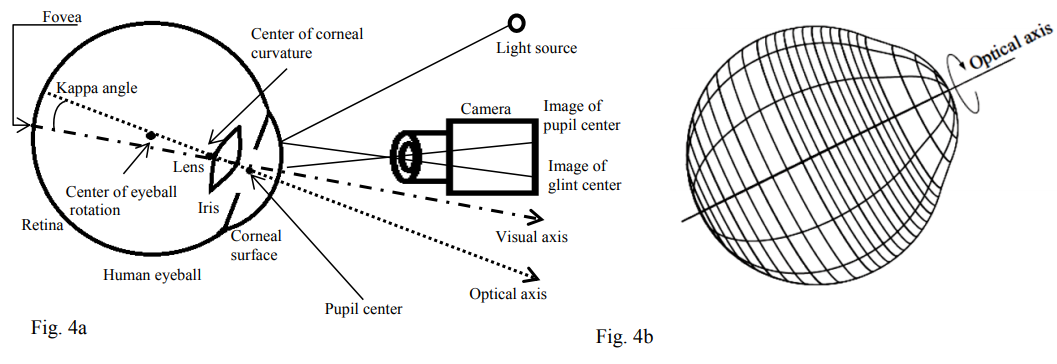
\includegraphics[scale=0.5]{img/Model_of_a_human_eye_ball.png}
    \end{center}
    \caption{Mô hình 3D: a. Mô hình bóng mắt người, thông số mắt và các yếu tố thiết lập được sử dụng trong theo dõi mắt 3D. Trục quang được hiển thị như là đường thẳng nối giữa tâm của giác mạc với trung tâm đồng tử mắt. Trục thị giác đi qua fovea và tâm của đường cong giác mạc. Góc Kappa là độ lệch góc giữa trục quang và thị giác. b. Một mô hình phi cầu của giác mạc, như một bề mặt của chuyển đổi về trục quang của mắt. \cite{AReviewandAnalysisofEyeGazeEstimation} }
    \label{refhinh15}
    \end{figure}
\end{center} 

\begin{center}
    \begin{figure}[h!]
    \begin{center}
     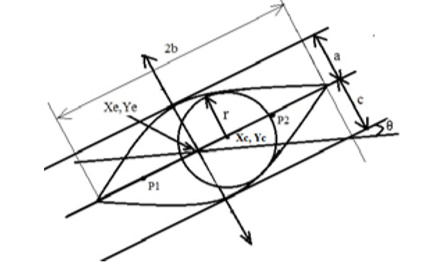
\includegraphics[scale=0.5]{img/Template_of_an_eye_region.PNG}
    \end{center}
    \caption{Phương pháp dựa trên hình dạng: Mẫu của một vùng mắt: Xc, Yc, Ye đại diện cho trung tâm của đồng tử và mắt tương ứng P1 và P2 là tiêu điểm của hai phần parabol và a, b, c và  là tham số, r là bán kính của đồng tử \cite{AReviewandAnalysisofEyeGazeEstimation}}
    \label{refhinh15}
    \end{figure}
\end{center}


\subsection{Chuẩn bị và xử lý dữ liệu}
Thu thập xử lý dữ liệu, tập dữ liệu sử dụng trong đề tài:
\begin{itemize}
\item Chuẩn bị tập dữ liệu  MPIIFaceGaze:\cite{dataset}

 Đối với bài toán phát hiện hướng nhìn, ban đầu nhận hình ảnh đầu vào là ảnh chỉ có mặt người mà không có nhiễu (không có các vật thể khác phía sau khuôn mặt). Tiếp theo đó xử lý hình ảnh để đánh nhãn ảnh hướng nhìn trên khuôn mặt, đưa vào mạng tiến hành training cho để đưa ra đầu ra cho hình ảnh bất kỳ.
 \begin{center}
    \begin{figure}[h!]
    \begin{center}
     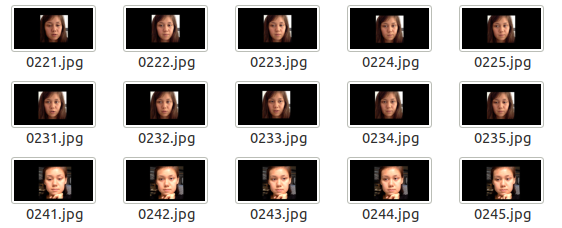
\includegraphics[scale=0.75]{img/MPIIFaceGaze-anh.png}
    \end{center}
    \caption{Tập dữ liệu ảnh MPIIFaceGaze.}
    \label{refhinh20}
    \end{figure}
\end{center}
 
%\section{Đề xuất cải tiến}
\end{itemize}
\begin{itemize}
\item Chuẩn bị tập dữ liệu  GazeCaptureEyeTracking:\cite{GazeCaptureEyeTracking}

 Bộ dữ liệu bao gồm dữ liệu cho các đối tượng duy nhất. Mỗi thư mục được đánh số đại diện cho một đối tượng. Các số được gán liên tục.

 \begin{center}
    \begin{figure}[h!]
    \begin{center}
     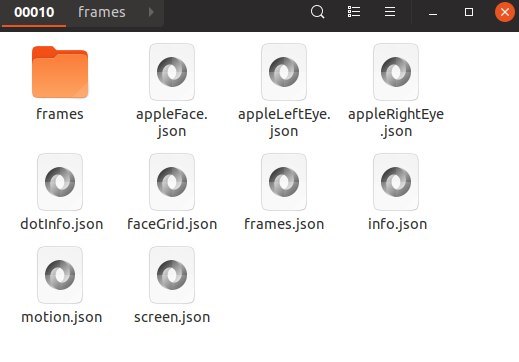
\includegraphics[scale=0.5]{img/GazeCaptureEyeTracking_JSon.png}
    \end{center}
    \caption{Tập dữ liệu ảnh GazeCaptureEyeTracking: thư mục frames chứa các file hình ảnh, và các file Json.}
    \label{refhinh20}
    \end{figure}
\end{center}

Bên trong mỗi thư mục là một tập hợp các hình ảnh được đánh số liên tục (trong thư mục con của thư mục frames) và các tệp JSON chứa thông tin cho các phần dữ liệu ảnh trong cùng thư mục. Nhiều biến trong các tệp JSON là các mảng, trong đó mỗi phần tử được liên kết với khung (frames) được đánh số giống như chỉ mục.
 \begin{center}
    \begin{figure}[h!]
    \begin{center}
     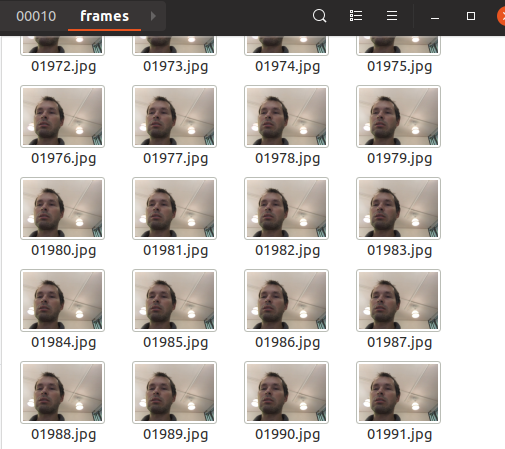
\includegraphics[scale=0.6]{img/GazeCaptureEyeTracking_anh.png}
    \end{center}
    \caption{Tập dữ liệu ảnh GazeCaptureEyeTracking: các file hình ảnh trong thư mục frames.}
    \label{refhinh20}
    \end{figure}
\end{center}

Thông tin các file Json:

 \textbf{+ appleFace.json, appleLeftEye.json, appleRightEye.json: }

Các tệp này mô tả các hộp giới hạn xung quanh khuôn mặt và mắt được phát hiện.  

X, Y: Vị trí của góc trên cùng bên trái của hộp giới hạn (tính bằng pixel).

W, H: Chiều rộng và chiều cao của khung giới hạn (tính bằng pixel).
\\

\textbf{+ dotInfo.json:}

    DotNum: Số thứ tự của dấu chấm (bắt đầu từ 0) được hiển thị trong khung đó.
    
     XPts, YPts: Vị trí trung tâm của dấu chấm (tính theo điểm; xem tài liệu screen.json bên dưới để biết thêm thông tin về đơn vị này) từ góc trên cùng bên trái của màn hình.
     
     XCam, YCam: Vị trí của tâm điểm trong không gian dự đoán của chúng tôi. Vị trí được đo bằng centimet và liên quan đến trung tâm camera, giả sử camera vẫn ở vị trí cố định trong không gian trên tất cả các hướng của thiết bị. Tức là, các giá trị YCam sẽ âm đối với các khung chế độ dọc (Định hướng == 1) vì màn hình nằm dưới camera, nhưng các giá trị sẽ dương ở chế độ chân dung lộn ngược (Định hướng == 2) vì màn hình nằm phía trên camera.
     
     Time: Thời gian (tính bằng giây) kể từ khi dấu chấm hiển thị xuất hiện lần đầu tiên trên màn hình.
\\

    
\textbf{+ faceGrid.json:}

    Các giá trị này mô tả các tính năng đầu vào "lưới mặt", được tạo ra từ các phát hiện khuôn mặt.
    X, Y: Vị trí của góc trên cùng bên trái của hộp mặt (được lập chỉ mục 1, trong lưới 25 x 25).
    
    W, H: Chiều rộng và chiều cao của hộp mặt.
    
    IsValid: Dữ liệu có hợp lệ (1) hay không (0).
 \\
   
    
\textbf{+ frames.json:}

Tên tệp của các khung (frames) trong thư mục khung. Thông tin này cũng có thể được tạo từ số thứ tự đếm từ 0 đến TotalFrames - 1 (xem info.json).
\\

\textbf{+ info.json:}

    TotalFrames: Tổng số khung cho chủ đề này.
    
     NumFaceDetections: Số lượng khung hình trong đó một khuôn mặt được phát hiện.
     
     NumEyeDetections: Số lượng khung hình trong đó mắt được phát hiện.
     
     Bộ dữ liệu: "đào tạo", "val" hoặc "kiểm tra" ("train," "val," or "test.")
     
     DeviceName: Tên của thiết bị được sử dụng trong bản ghi.
\\
    
\textbf{+ motion.json, screen.json:}

Thông tin về  luồng dữ liệu chuyển động và định hướng của giao diện
%\section{Đề xuất cải tiến}
\end{itemize}


\section{Tiến hành thực hiện}

	Từ những bức ảnh chụp khuôn mặt người thông qua các mô hình có thể phát hiện ra hướng cửa mắt. Nhóm chia hướng nhìn của mắt làm 9 hướng và nhắm mắt.

\begin{center}
    \begin{figure}[h!]
    \begin{center}
     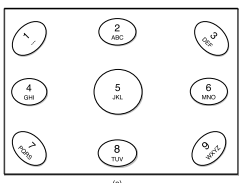
\includegraphics[scale=0.8]{img/direction.png}
    \end{center}
    \caption{Các hướng nhìn \cite{9direction}}
    \label{refhinh21}
    \end{figure}
\end{center}



\newpage 
\subsection{Tập dữ liệu GazeCaptureEyeTracking}
Phương pháp sử dụng học sâu với mô hình CNNs: Từ tập  hình ảnh với các tệp dữ liệu json , tiến hành training cho để đưa ra kết quả. Mô hình đã thực hiện với cấu hình sau:

    Python 3.6.7
    
    OpenCV 3.4.4
    
    Keras 2.2.4
    
    TensorFlow 1.11.0

 \begin{center}
    \begin{figure}[h!]
    \begin{center}
     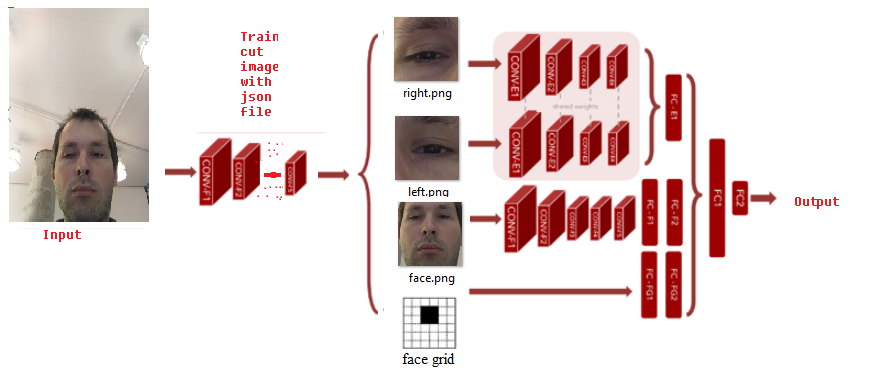
\includegraphics[scale=0.7]{img/mohinhtrain1.png}
    \end{center}
    \caption{Mô hình CNNs sử dụng training tập dữ liệu GazeCaptureEyeTracking.}
    \label{refhinh20}
    \end{figure}
\end{center}


 \begin{center}
    \begin{figure}[h!]
    \begin{center}
     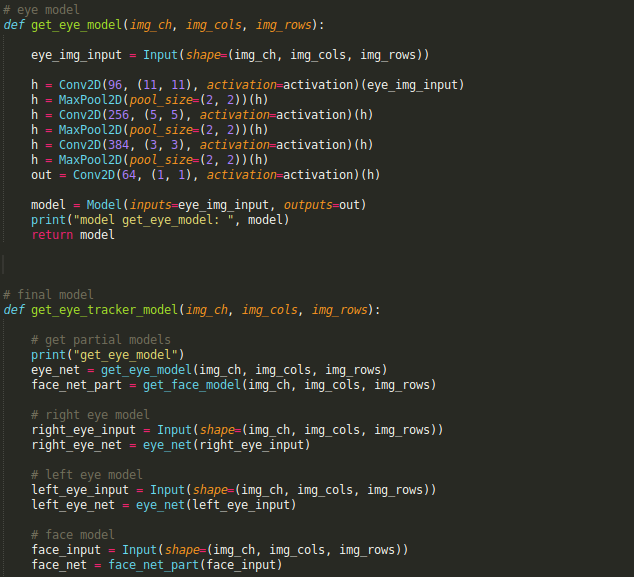
\includegraphics[scale=0.5]{img/mohindetect.png}
    \end{center}
    \caption{Mô hình (model) thực hiện phát hiện ánh nhìn}
    \label{refhinh20}
    \end{figure}
\end{center}

 \begin{center}
    \begin{figure}[h!]
    \begin{center}
     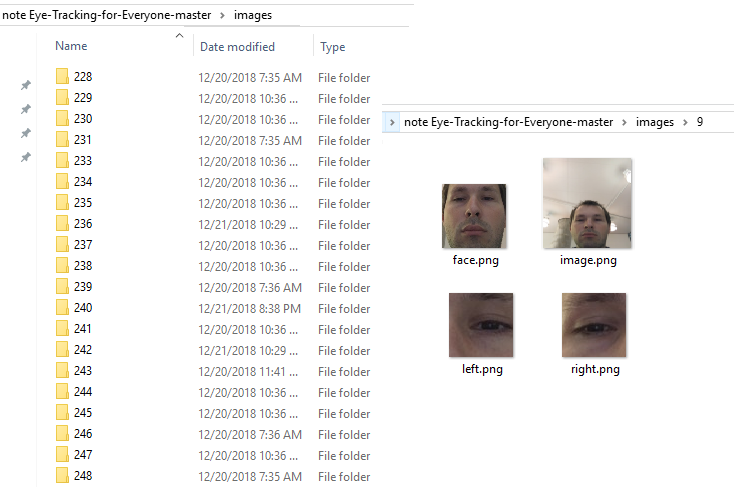
\includegraphics[scale=0.6]{img/5fileanhchupoutputthumuc1.png}
    \end{center}
    \caption{Kết quả nhận được tập ảnh chứa các hình ảnh cắt mắt phải, trái}
    \label{refhinh20}
    \end{figure}
\end{center}

\newpage
\subsection{Tập dữ liệu MPIIFaceGaze}

Sử dụng kết hợp mô hình đơn giản linear model để train: Xử lý hình ảnh đánh nhãn ảnh khuôn mặt, tiến hành training cho để đưa ra kết quả. Một số kết quả nhận được:
 \begin{center}
    \begin{figure}[h!]
    \begin{center}
     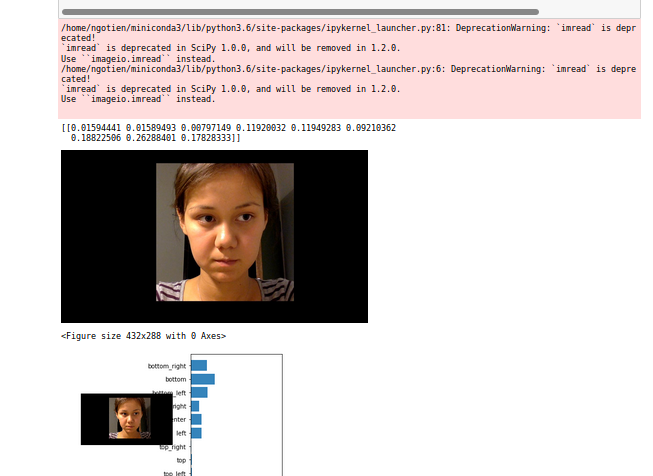
\includegraphics[scale=0.6]{img/MPIIFaceGaze-anh-dau-co-ten-file.png}
    \end{center}
    \caption{Kết quả thu được (dữ liệu ảnh MPIIFaceGaze).}
    \label{refhinh20}
    \end{figure}
\end{center}

 \begin{center}
    \begin{figure}[h!]
    \begin{center}
     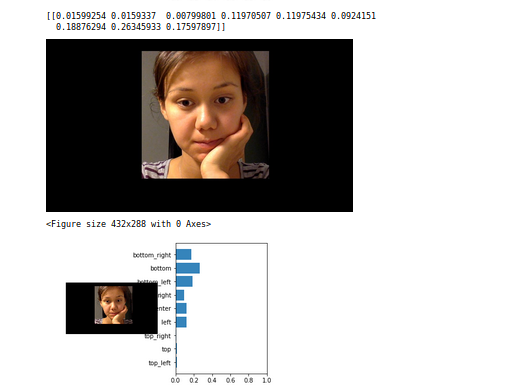
\includegraphics[scale=0.75]{img/MPIIFaceGaze-anh-ket-qua1.png}
    \end{center}
    \caption{Tập dữ liệu ảnh MPIIFaceGaze.}
    \label{refhinh20}
    \end{figure}
\end{center}
\clearpage 

\section{Đánh giá kết quả, mô hình}
Trong quá trình nghiên cứu, tôi đã:
\begin{itemize}
\item Hiểu được căn bản và cách hoạt động của mạng CNN.

\item Hiểu được kiến trúc nâng cao của mạng CNN cũng như các vấn đề và cách giải quyết

\item Tổng hợp, đánh giá ưu và nhược điểm của cách phương pháp, công nghệ đã và đang được nghiên cứu, sử dụng. 

\item Tiếp cận vấn đề theo nhiều hướng khác nhau, các nghiên cứu kỹ thuật dõi chuyển động mắt hiện nay

\item Thực hiện một số phương pháp sử dụng học sâu (CNN) để phát hiện hướng nhìn của con người qua hình ảnh nhưng độ chính xác chưa cao do đòi hỏi  yêu cầu kỹ thuật cao (Kỹ năng phân tích hình dạng mắt, Mô hình 3D, Camera,...)

\item Cuối cùng, tôi đề xuất hướng phát triển tiếp theo của đề tài trong tương lai: Phân tích hình ảnh mắt, cấu trúc mắt đồng tử, điều chỉnh hướng camera,... tăng độ chính xác của kết quả, phát triển thành ứng dụng trên thiết bị máy tính, điện thoại có thể giúp người khuyết tật điều khiển các thiết bị chỉ bằng ánh mắt mà không cần đến đôi tay, theo dõi người lái xe có thể phát hiện kịp thời người này ngủ gật hay không chú ý khi lái xe,...
\end{itemize}